\documentclass[]{book}

%These tell TeX which packages to use.
\usepackage{array,epsfig}
\usepackage{amsmath}
\usepackage{amsfonts}
\usepackage{amssymb}
\usepackage{amsxtra}
\usepackage{amsthm}
\usepackage{mathrsfs}
\usepackage{color}
\usepackage{algorithm}
\usepackage{MnSymbol}
\usepackage{tikz}
\usetikzlibrary{cd,automata, positioning}
\usepackage[noend]{algpseudocode}

%Here I define some theorem styles and shortcut commands for symbols I use often
\theoremstyle{definition}
\newtheorem{defn}{Definition}
\newtheorem{thm}{Theorem}
\newtheorem{cor}{Corollary}
\newtheorem*{rmk}{Remark}
\newtheorem{lem}{Lemma}
\newtheorem*{joke}{Joke}
\newtheorem{ex}{Example}
\newtheorem*{soln}{Solution}
\newtheorem{prop}{Proposition}

\newcommand{\lra}{\longrightarrow}
\newcommand{\ra}{\rightarrow}
\newcommand{\surj}{\twoheadrightarrow}
\newcommand{\graph}{\mathrm{graph}}
\newcommand{\bb}[1]{\mathbb{#1}}
\newcommand{\Z}{\bb{Z}}
\newcommand{\Q}{\bb{Q}}
\newcommand{\R}{\bb{R}}
\newcommand{\C}{\bb{C}}
\newcommand{\N}{\bb{N}}
\newcommand{\M}{\mathbf{M}}
\newcommand{\m}{\mathbf{m}}
\newcommand{\MM}{\mathscr{M}}
\newcommand{\HH}{\mathscr{H}}
\newcommand{\Om}{\Omega}
\newcommand{\Ho}{\in\HH(\Om)}
\newcommand{\bd}{\partial}
\newcommand{\del}{\partial}
\newcommand{\bardel}{\overline\partial}
\newcommand{\textdf}[1]{\textbf{\textsf{#1}}\index{#1}}
\newcommand{\img}{\mathrm{img}}
\newcommand{\ip}[2]{\left\langle{#1},{#2}\right\rangle}
\newcommand{\inter}[1]{\mathrm{int}{#1}}
\newcommand{\exter}[1]{\mathrm{ext}{#1}}
\newcommand{\cl}[1]{\mathrm{cl}{#1}}
\newcommand{\ds}{\displaystyle}
\newcommand{\vol}{\mathrm{vol}}
\newcommand{\cnt}{\mathrm{ct}}
\newcommand{\osc}{\mathrm{osc}}
\newcommand{\LL}{\mathbf{L}}
\newcommand{\UU}{\mathbf{U}}
\newcommand{\support}{\mathrm{support}}
\newcommand{\AND}{\;\wedge\;}
\newcommand{\OR}{\;\vee\;}
\newcommand{\Oset}{\varnothing}
\newcommand{\st}{\ni}
\newcommand{\wh}{\widehat}

%Pagination stuff.
\setlength{\topmargin}{-.3 in}
\setlength{\oddsidemargin}{0in}
\setlength{\evensidemargin}{0in}
\setlength{\textheight}{9.in}
\setlength{\textwidth}{6.5in}
\pagestyle{empty}


\makeatletter
\def\BState{\State\hskip-\ALG@thistlm}
\makeatother



\begin{document}
	
	\section*{Modifizierte Wassersteindistanz}
	
	Um die Wasserstein Distanz für nicht gleichgroße Knotenmengen zu erweitern, betrachten wir folgendes für $X$ und $Y$ zwei Punktmengen oberhalb der Diagonalen $\Delta=\{(x,x)\in\mathbb{R}^2 | x \in \mathbb{R}\}$, mit $|X|<|Y|$:
	
	$$W(X,Y):=\inf_{\varphi:X\hookrightarrow Y}\bigg(\sum_{x\in X}||x-\varphi(x)|| + \sum_{y\in Y\setminus im(\varphi)}\gamma(y) \bigg)$$
	
	wobei $\varphi$ injektiv sein soll, und man $\gamma:\mathbb{R}^2\rightarrow\mathbb{R}$ z.B. definieren als die "Lebensdauer" des Punktes, also $\gamma(x,y) = y-x$. Alternativ auch der minimale Abstand von dem Punkt $(x,y)$ zu der Diagonalen $\Delta$. Allerdings ist dieser Abstand einfach $\frac{y-x}{\sqrt{2}}$, also ein Skalar von dem anderen Abstand. Dieser Abstand $W(X,Y)$ lässt sich interpretieren als die normale Wasserstein Distanz, wobei alle Punkte in der Zielmenge, die nicht im Bild von $\varphi$ enthalten sind, getroffen werden von einem Punkt auf der Diagonalen, die keinen Mehrwert für die persistente Homologie haben.
	
	Diese Alternative respektiert die Wichtigkeit jedes einzelnen Punktes, insbesondere den "lange lebenden". Die Wasserstein Distanz so zu erweitern ergibt natürlich nur im Zusammenhang mit persistenter Homologie Sinn. Eine andere Methode, die ich aber schon verworfen habe, ist erst auf der Menge $Y$ ein $|X|$-Clustering $C$ zu finden, und dann über die Mappings $X\rightarrow C$ zu optimieren. Hierbei verliert man aber wichtige Details, wenn zwei Punkte die "lange leben", und zeitgleich geboren werden z.B. zu einem Cluster werden. Dadurch verliert man eine wichtige Information über einen Erzeuger der ersten Homologie.
	
	\subsection*{Effiziente Berechnung}
	
	Das ganze lässt sich polynomiell lösen. Hierbei reduziert man das Problem auf eine min-cost-flow-Instanz. Gegeben $X$ mit $|X|=k$ und $Y$ mit $|Y|=n>k$. Dann definieren wir einen Graphen $G = (V,E)$, wobei $V=X\cup\{s,t,h\}$. $s$,$t$ und $h$ sind hierbei Hilfsknoten. Die Menge der Kanten besteht aus der Vereinigung von $\{(s,a)|a\in X\cup\{h\}\}$, $\{(a,b)|a\in X\cup\{h\},b\in Y\}$ und $\{(b,t)|b\in Y\}$. Die Kapazitäten $u:E\rightarrow \mathbb{R}$ definieren wir hierbei als $n-k$ für alle Kanten der Form $(h,y)$ mit $y\in Y$ und die Kante $(s,h)$, und $1$ für alle anderen Kanten. Die Kosten für Kanten der Form $(x,y)$ mit $x\in X$ und $y\in Y$ sei $||x-y||$. Die Kosten für Kanten der Form $(h,y)$ mit $y\in Y$ sei der oben beschriebene Abstand $\gamma(y)$. Alle anderen Kosten sind $0$. Und Flow-Variablen $b(s) = -b(t) = n$, $b(v) = 0$ für alle anderen $v$. Gesucht wird jetzt ein min-cost-flow. Dieser ist optimal lösbar in polynomieller Zeit durch z.B. einen Algorithmus wie Cycle-Cancling. Weil die Kapazitäten alle ganzzahlig sind, ist die Lösung auch ganzzahlig, und somit können wir einfach gucken welche Kanten ausgewählt wurden, welches dann die optimale Abbildung $\varphi$ bestimmt. Sogar genauer, $W(X,Y)$ ist dann genau gleich dem Gewicht der optimalen Lösung. Hier beispielhaft der Graph $G$ ohne Kosten und Kapazitäten für $k=2$ und $n=4$.
	
	\begin{figure}[!h]
		\centering
	\begin{tikzpicture}
	\node[shape=circle,draw=black] (A) at (0,0) {$s$};
	\node[shape=circle,draw=black] (B) at (2.5,2) {$x_1$};
	\node[shape=circle,draw=black] (C) at (2.5,0) {$x_2$};
	\node[shape=circle,draw=black] (D) at (2.5,-2) {$h$};
	\node[shape=circle,draw=black] (E) at (5,3) {$y_1$};
	\node[shape=circle,draw=black] (F) at (5,1) {$y_2$};
	\node[shape=circle,draw=black] (G) at (5,-1) {$y_3$} ;
	\node[shape=circle,draw=black] (H) at (5,-3) {$y_4$} ;
	\node[shape=circle,draw=black] (I) at (7.5,0) {$t$} ;
	
	\path [->] (A) edge node {} (B);
	\path [->] (A) edge node {} (C);
	\path [->] (A) edge node {} (D);
	
	
	\path [->] (B) edge node {} (E);
	\path [->] (B) edge node {} (F);
	\path [->] (B) edge node {} (G);
	\path [->] (B) edge node {} (H);
	
	\path [->] (C) edge node {} (E);
	\path [->] (C) edge node {} (F);
	\path [->] (C) edge node {} (G);
	\path [->] (C) edge node {} (H);
	
	\path [->] (D) edge node {} (E);
	\path [->] (D) edge node {} (F);
	\path [->] (D) edge node {} (G);
	\path [->] (D) edge node {} (H);
	
	\path [->] (E) edge node {} (I);
	\path [->] (F) edge node {} (I);
	\path [->] (G) edge node {} (I);
	\path [->] (H) edge node {} (I); 
	\end{tikzpicture} 
	\end{figure}
	
\end{document}


